\hypertarget{what-is-agile-architecture}{%
\section{What is Agile Architecture?}\label{what-is-agile-architecture}}

Every programmer is some kind of architect --whether wanted or not.
Every act of programming is some kind of architectural act -- good or
bad, small or large, intended or not --.

\hypertarget{some-agile-manifesto-principles}{%
\subsection{Some Agile Manifesto
Principles}\label{some-agile-manifesto-principles}}

\begin{itemize}
\tightlist
\item
  Our highest priority is to satisfy the customer through early and
  continuous delivery of valuable software.
\item
  Business people and developers must work together daily throughout the
  project.
\item
  Build projects around motivated individuals. Give them the environment
  and support they need, and trust them to get the job done.
\item
  Working software is the primary measure of progress.
\item
  Continuous attention to technical excellence and good design enhances
  agility.
\item
  Simplicity - the art of maximizing the amount of work not done - is
  essential.
\item
  The best architectures, requirements, and designs emerge from
  self-organizing teams.
\end{itemize}

\hypertarget{agile-architecture-principles-safe}{%
\subsection{Agile Architecture Principles
(SAFe)}\label{agile-architecture-principles-safe}}

\begin{enumerate}
\def\labelenumi{\arabic{enumi}.}
\tightlist
\item
  Design emerges. Architecture is a collaboration.
\item
  The bigger the system, the longer the runway.
\item
  Build the simplest architecture that can possibly work.
\item
  When in doubt, code or model it out.
\item
  They build it. They test it, They run it.
\item
  There is no monopoly on innovation.
\item
  Implement architectural flow.
\end{enumerate}



\subsubsection{Spike}
When you Spike you prove if an idea working or not. But not for long, give yourself a restriction to hours or days, not weeks!
\begin{figure}[H]
\centering
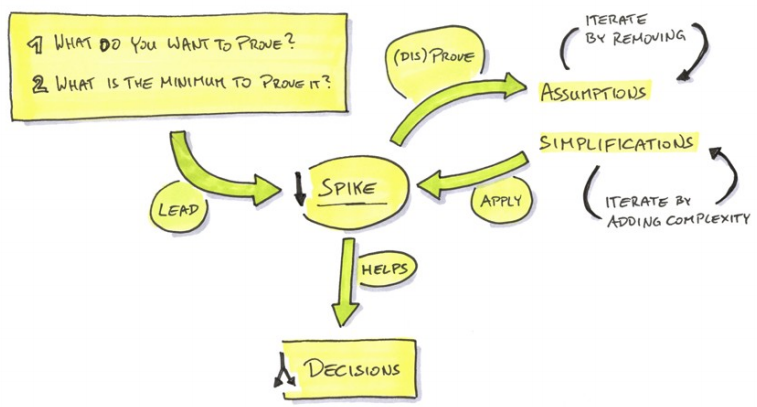
\includegraphics[width=0.5\textwidth]{figures/Spike.PNG}
\caption{Spike Process}
\end{figure}



\clearpage